\documentclass[a4paper,12pt]{extarticle}
\usepackage{geometry}
\usepackage[T1]{fontenc}
\usepackage[utf8]{inputenc}
\usepackage[english,russian]{babel}
\usepackage{amsmath}
\usepackage{amsthm}
\usepackage{amssymb}
\usepackage{fancyhdr}
\usepackage{setspace}
\usepackage{graphicx}
\usepackage{colortbl}
\usepackage{tikz}
\usepackage{pgf}
\usepackage{subcaption}
\usepackage{listings}
\usepackage{indentfirst}
\usepackage{float}

\usepackage[
backend=biber,
style=numeric,
maxbibnames=99
]{biblatex}
\addbibresource{refs.bib}
\usepackage[colorlinks,citecolor=blue,linkcolor=blue,bookmarks=false,hypertexnames=true, urlcolor=blue]{hyperref} 
\usepackage{indentfirst}
\usepackage{mathtools}
\usepackage{booktabs}
\usepackage[flushleft]{threeparttable}
\usepackage{tablefootnote}

\usepackage{chngcntr} % нумерация графиков и таблиц по секциям
\counterwithin{table}{section}
\counterwithin{figure}{section}

\graphicspath{{graphics/}}%путь к рисункам

\makeatletter
% \renewcommand{\@biblabel}[1]{#1.} % Заменяем библиографию с квадратных скобок на точку:
\makeatother

\geometry{left=2.5cm}% левое поле
\geometry{right=1.0cm}% правое поле
\geometry{top=2.0cm}% верхнее поле
\geometry{bottom=2.0cm}% нижнее поле
\setlength{\parindent}{1.25cm}
\renewcommand{\baselinestretch}{1.5} % междустрочный интервал


\newcommand{\bibref}[3]{\hyperlink{#1}{#2 (#3)}} % biblabel, authors, year
\addto\captionsrussian{\def\refname{Список литературы (или источников)}} 

\renewcommand{\theenumi}{\arabic{enumi}}% Меняем везде перечисления на цифра.цифра
\renewcommand{\labelenumi}{\arabic{enumi}}% Меняем везде перечисления на цифра.цифра
\renewcommand{\theenumii}{.\arabic{enumii}}% Меняем везде перечисления на цифра.цифра
\renewcommand{\labelenumii}{\arabic{enumi}.\arabic{enumii}.}% Меняем везде перечисления на цифра.цифра
\renewcommand{\theenumiii}{.\arabic{enumiii}}% Меняем везде перечисления на цифра.цифра
\renewcommand{\labelenumiii}{\arabic{enumi}.\arabic{enumii}.\arabic{enumiii}.}% Меняем везде перечисления на цифра.цифра

\begin{document}
\input{title_kr}% это титульный лист - выберите подходящий вам из имеющихся в проекте вариантов (kr - курсовая работа у 3 курса, vkr - выпускная квалификационная работа у 4 курса)
\newpage
\setcounter{page}{2}

{
	\hypersetup{linkcolor=black}
	\tableofcontents
}

\newpage

\newpage
\section*{Аннотация}   % this is how to use russian
В последние годы широкое распространение получили подходы к планированию движений манипуляторов, основанные на разбиении пространства конфигураций на граф выпуклых регионов и последующей оптимизации по этому графу. Ключевым узким местом таких методов является построение выпуклых областей в пространстве высокой размерности. Этот этап требует значительных вычислительных затрат, а полученные регионы не всегда обладают хорошими геометрическими свойствами, что приводит к ухудшению качества графа и увеличению времени поиска траектории.

В данной работе проводится исследование различных способов построения графа выпуклых оболочек в пространстве конфигураций манипулятора и анализируется их влияние на длину планируемого пути и время построения разбиения.

\addcontentsline{toc}{section}{Аннотация}

\section*{Ключевые слова}
Планирование движений, робот-манипулятор, пространство конфигураций, выпуклые области, граф выпуклых оболочек
\pagebreak

\addcontentsline{toc}{section}{Ключевые слова}

\section{Введение}
Планирование движений для робототехнических манипуляторов в среде с
препятствиями является важной задачей для промышленной 
робототехники. Требуется построить траекторию в пространстве
конфигураций, удовлетворяющую ограничениям на коллизии и движения
робота, при этом практическая применимость определяется как качеством
траектории, так и вычислительной стоимостью планирования.

В работе рассматривается семейство методов, основанных на
представлении свободного пространства в виде графа выпуклых множеств
(Graph of Convex Sets, GCS), и анализируется влияние способов
построения данного представления на качество решений и вычислительные
затраты при планировании движений манипулятора.
Задача выбора и сравнения способов построения графа выпуклых оболочек остаётся открытой. В частности, не до конца исследованным является влияние различных методов разбиения пространства конфигураций на качество планируемых траекторий и вычислительную эффективность алгоритмов планирования, что и является предметом настоящей работы.

\section{Обзор работ в предметной области}
Задача планирования движений в пространствах высокой размерности является широко исследуемой задачей на протяжении последних десятилетий и имеет множество подходов.
Основные из них можно разделить на следующие группы:
\begin{enumerate}
    \item Sampling-based подходы
    \item Optimization-based подходы
    \item Learning-based подходы
\end{enumerate}
Каждый из перечисленных подходов обладает собственными
преимуществами и ограничениями, что приводит к активному
развитию гибридных методов, сочетающих идеи нескольких парадигм для
повышения масштабируемости и надёжности планирования в сложных сценариях.

\subsection{Sampling-based подходы}
Методы планирования движений, основанные на случайном семплировании
конфигурационного пространства, получили широкое распространение
благодаря своей применимости в пространствах высокой размерности и
наличию формальных теоретических свойств. К числу базовых алгоритмов
данного класса относятся PRM (Probabilistic Roadmaps)~\cite{2} и RRT
(Rapidly Exploring Random Trees)~\cite{1}, которые заложили основу для большинства
современных sampling-based подходов.

В последующих работах было предложено множество модификаций указанных
алгоритмов, направленных на повышение вычислительной эффективности и
качества получаемых решений. В частности, в широко используемых
программных библиотеках, таких как OMPL (Open Motion Planning Library)~\cite{8},
реализованы различные варианты алгоритма RRT, включая RRT*~\cite{2}, обладающий
свойством асимптотической оптимальности за счёт переоптимизации
локальных соединений, а также RRT-Connect~\cite{9}, использующий двунаправленный
рост деревьев для ускорения поиска допустимого пути.
Ключевым теоретическим свойством sampling-based методов является
\emph{probabilistic completeness}, означающая, что при существовании
допустимого решения вероятность того, что алгоритм не сможет его найти,
стремится к нулю по мере увеличения числа сэмплов
~\cite{11},~\cite{12}.

Для алгоритмов семейства RRT* дополнительно показана асимптотическая
оптимальность, то есть сходимость стоимости найденного пути к
оптимальному решению при неограниченном росте числа сэмплов.
Более строгий анализ условий выполнения данных гарантий, а также
уточнение исходного доказательства асимптотической оптимальности
RRT* представлены в работе~\cite{10}.

При этом следует отметить, что указанные теоретические гарантии носят
асимптотический характер и не обеспечивают нахождение решения за
конечное время, что может существенно ограничивать практическую
эффективность sampling-based методов в задачах планирования движений
для манипуляторов в пространствах высокой размерности.

\subsection{Optimization-based подходы}
Несмотря на наличие формальных теоретических гарантий, sampling-based
методы обладают рядом практических ограничений, связанных с высокой вычислительной
стоимостью и ограниченным качеством получаемых траекторий. В
частности, такие методы, как правило, находят лишь геометрически
допустимый путь, который требует дополнительной постобработки для
обеспечения гладкости и соответствия кинематическим ограничениям
манипулятора. Эти недостатки послужили мотивацией для развития
optimization-based подходов к планированию движений.

Optimization-based методы формулируют задачу планирования движений как
задачу оптимизации в непрерывном пространстве траекторий, где
необходимо минимизировать функционал стоимости при наличии
ограничений, отражающих требования к коллизиям, гладкости траектории и
ограничениям на движения робота~\cite{17}. В рамках данного подхода траектория
обычно параметризуется конечным числом переменных, а поиск решения
осуществляется с использованием численных методов
оптимизации~\cite{18}.

К числу наиболее известных optimization-based алгоритмов относятся
CHOMP~\cite{13}, STOMP~\cite{14} и TrajOpt~\cite{15}, которые получили широкое распространение в
задачах планирования движений для робототехнических манипуляторов.
Данные методы позволяют напрямую учитывать требования к гладкости и
динамическим характеристикам движения, что делает их особенно
привлекательными для практического применения. Однако в задачах оптимизации
качество найденного решения сильно зависит от начальной инициализации
траектории, что подробно обсуждается в~\cite{16}.

Существенным отличием optimization-based подходов от sampling-based
методов является отсутствие глобальных гарантий нахождения решения в
случае его существования. В отличие от probabilistic completeness,
характерной для sampling-based алгоритмов, optimization-based методы
обеспечивают лишь локальную оптимальность и могут сходиться к
недопустимым или субоптимальным решениям~\cite{15}.

\subsection{Learning-based подходы}
Learning-based подходы к планированию движений используют методы
машинного обучения для повышения эффективности классических
sampling-based и optimization-based алгоритмов. В отличие от
традиционных методов, такие подходы, как правило, не предоставляют
строгих теоретических гарантий корректности и сходимости, однако
позволяют существенно сократить время планирования и повысить
масштабируемость в пространствах высокой размерности~\cite{19}.

Наиболее распространённым сценарием применения learning-based методов
является их использование в качестве вспомогательных компонентов
планировщика. В частности, обучаемые модели применяются для генерации
информативных сэмплов и направленного расширения деревьев поиска, что
позволяет ускорить sampling-based планирование без нарушения его
базовых свойств~\cite{20}~\cite{21}.

Другим направлением является использование нейронных моделей для
приближённого предсказания допустимости соединений между
конфигурациями, а также для обучения структурированных представлений
пространства конфигураций, что снижает вычислительные затраты при
построении траекторий~\cite{22}~\cite{23}.

Несмотря на достигнутые успехи, learning-based подходы остаются
чувствительными к качеству обучающих данных и демонстрируют ограниченную
обобщающую способность за пределами распределения обучающей выборки. В
связи с этим на практике наибольший интерес представляют гибридные
методы, в которых learning-based компоненты используются совместно с
классическими алгоритмами планирования для сохранения надёжности и
интерпретируемости решений~\cite{21}~\cite{23}.


\section{Обзор литературы}
Классические подходы к планированию движений характеризуются различными
компромиссами между вычислительной сложностью и качеством решений. Одним
из направлений, сочетающих дискретный выбор структуры решения с
непрерывной оптимизацией, является подход Graphs of Convex Sets (GCS).

Подход Graphs of Convex Sets (GCS)~\cite{5} формулирует задачу планирования
движений как поиск пути на графе, вершины которого соответствуют
выпуклым подмножествам допустимого пространства, а рёбра задают
возможность перехода между ними. В рамках данного подхода дискретный
выбор последовательности регионов сочетается с непрерывной оптимизацией
внутри каждого выпуклого множества.

Ключевой проблемой при применении GCS является построение набора
выпуклых регионов, лежащих целиком в свободном от коллизий пространстве
конфигураций. В работах, основанных на методе IRIS~\cite{6}, предлагается
строить большие выпуклые области без коллизий с использованием выпуклой оптимизации~\cite{24}.
Развитие данного подхода в виде C-IRIS позволяет получать
сертифицированные выпуклые регионы в пространстве конфигураций
манипуляторов, однако вычислительная сложность таких методов быстро
возрастает с увеличением размерности задачи~\cite{25}.

В более поздних работах рассматриваются приближённые и масштабируемые
методы построения GCS, направленные на уменьшение числа выпуклых
регионов и ускорение их построения. В ~\cite{7}, предлагается
аппроксимировать пространство конфигураций с использованием покрытий
графа видимости кликами.


\section{Эксперименты}

В данном разделе представлены результаты экспериментального исследования,
направленного на анализ качества разбиения пространства конфигураций на
выпуклые регионы, а также на оценку влияния этого разбиения на эффективность
планирования траекторий с использованием графа выпуклых множеств (GCS).

\subsection{Эксперименты по построению выпуклых регионов}

В первой серии экспериментов исследовалось влияние способа генерации
начальных точек для алгоритма IRIS на качество разбиения пространства
конфигураций. Качество разбиения напрямую влияет на эффективность поиска
в задачах GCS, поскольку узкие, вытянутые или слабо связанные выпуклые
регионы приводят к ухудшению сходимости алгоритмов оптимизации.

Для построения выпуклых регионов использовалась реализация алгоритма IRIS
из симулятора Drake. В качестве тестовой платформы применялась модель
манипулятора KUKA iiwa с 7 степенями свободы. Эксперименты проводились в
трёх сценах различной сложности: сцена с одной полкой, сцена с двумя
параллельными полками и сцена с тремя полками, расположенными вокруг
манипулятора (Рис. 2.1).

\begin{figure}[H]
    \centering

    \begin{subfigure}[t]{0.32\textwidth}
        \centering
        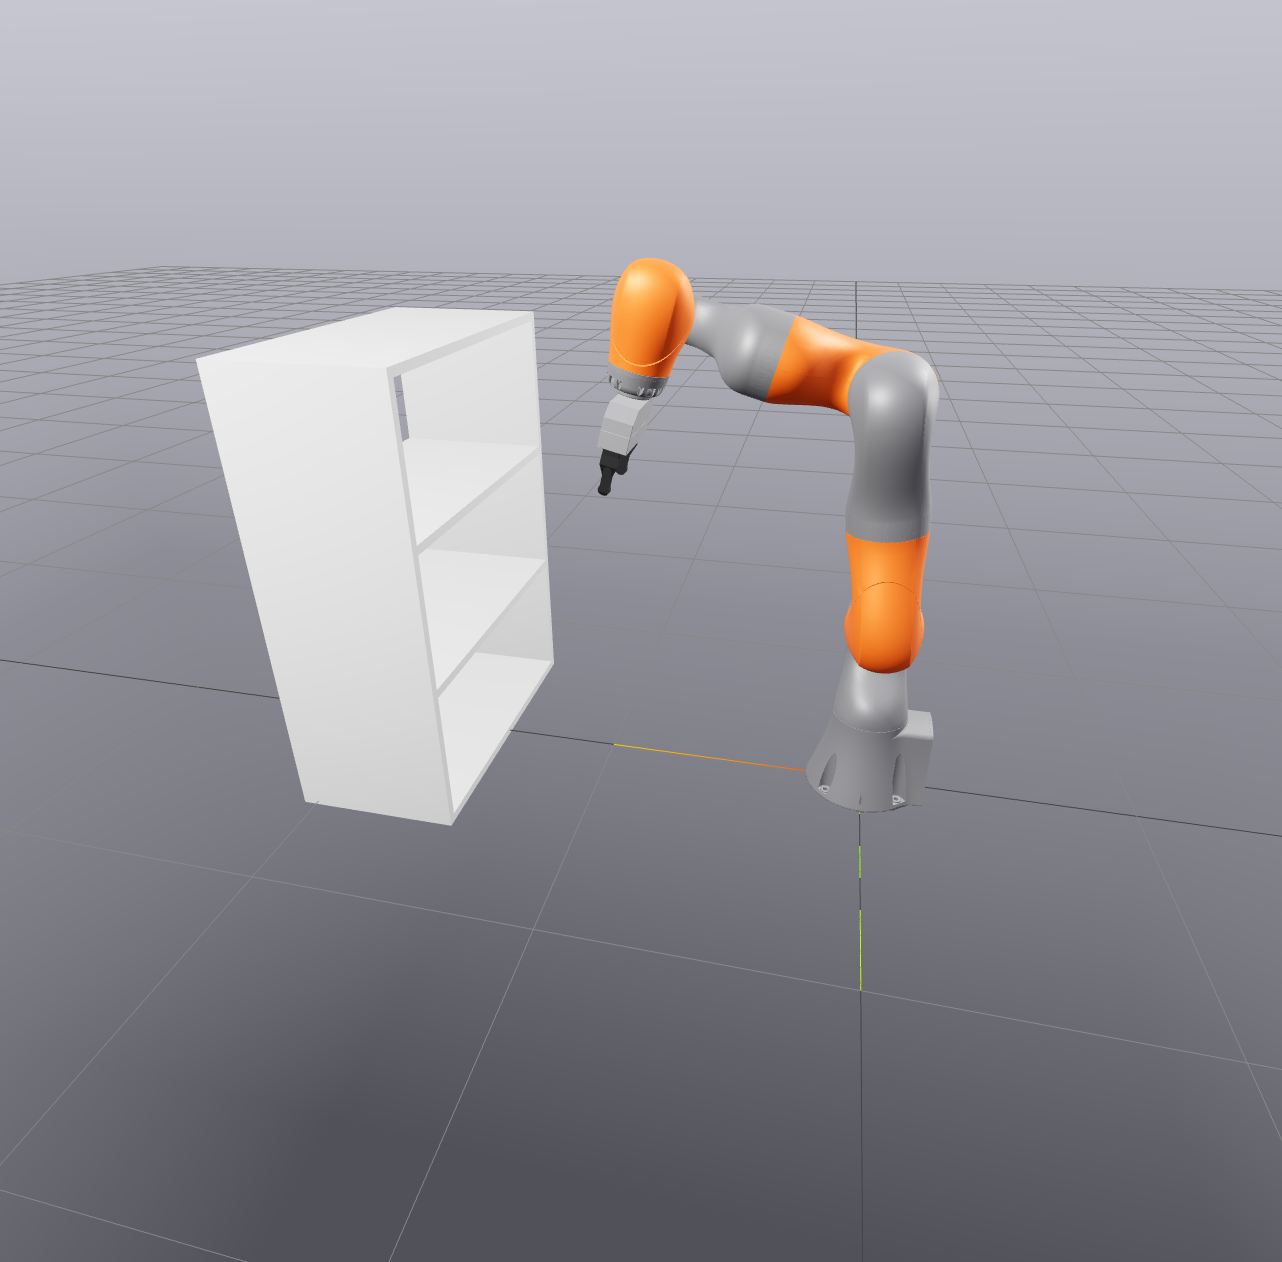
\includegraphics[
            height=3.5cm,
            keepaspectratio
        ]{meshcat1.png}
        \caption{Манипулятор и одна полка}
    \end{subfigure}
    \hfill
    \begin{subfigure}[t]{0.32\textwidth}
        \centering
        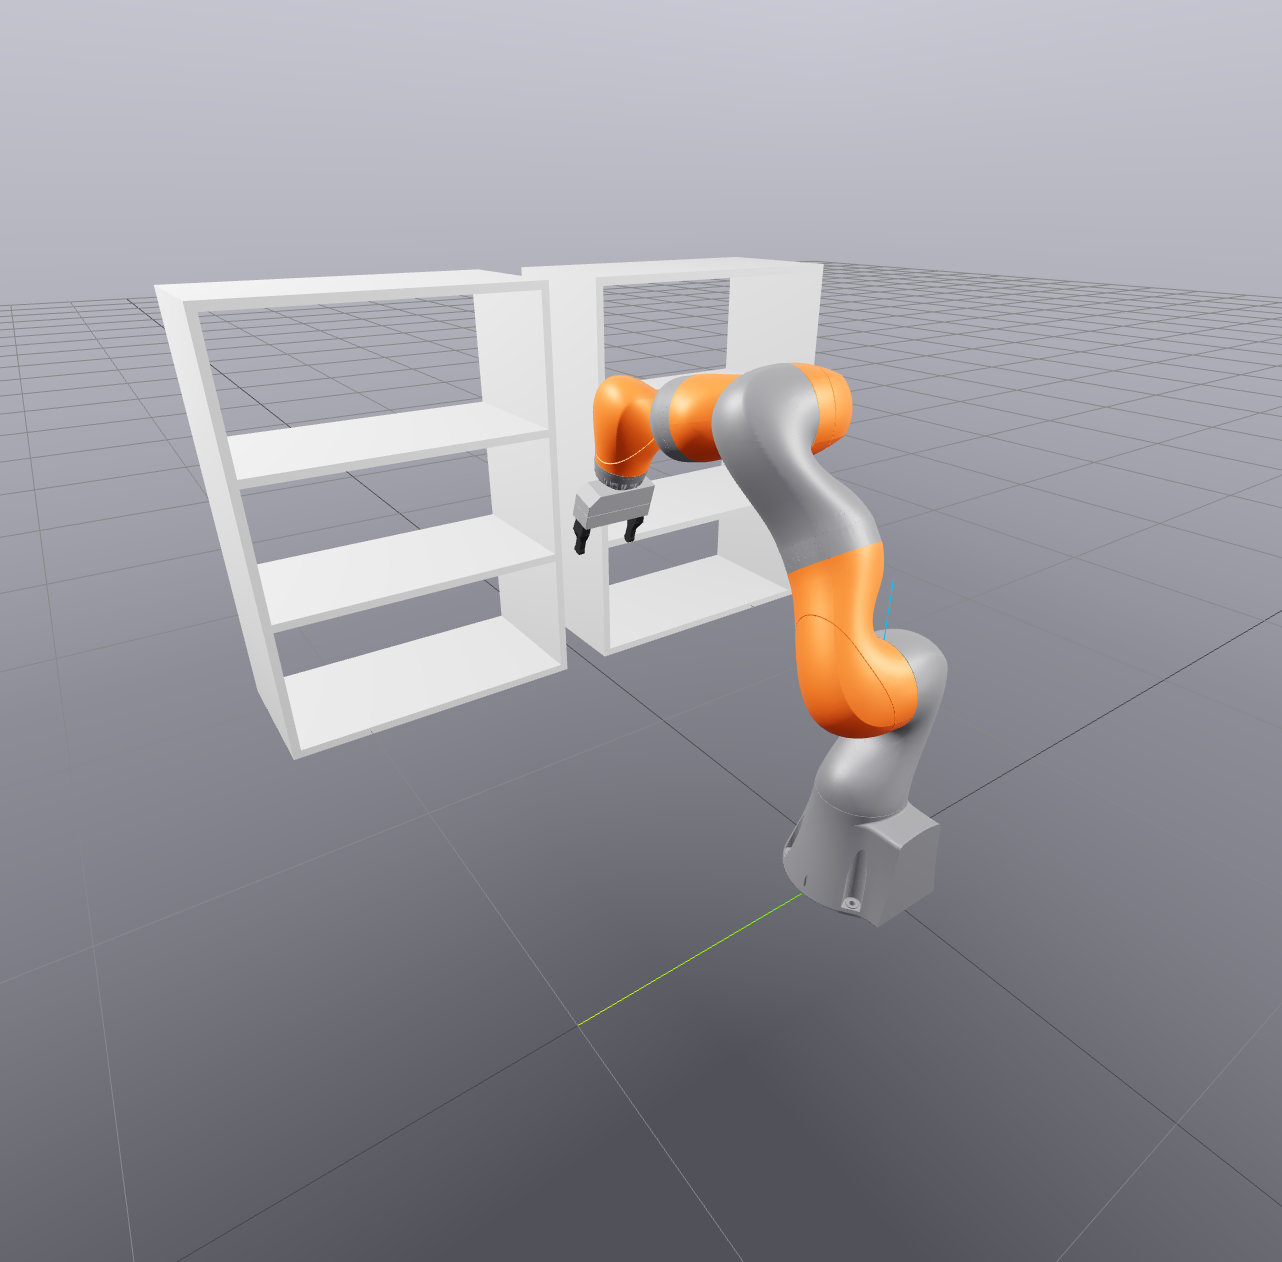
\includegraphics[
            height=3.5cm,
            keepaspectratio
        ]{meshcat2.png}
        \caption{Манипулятор и две параллельные полки}
    \end{subfigure}
    \hfill
    \begin{subfigure}[t]{0.32\textwidth}
        \centering
        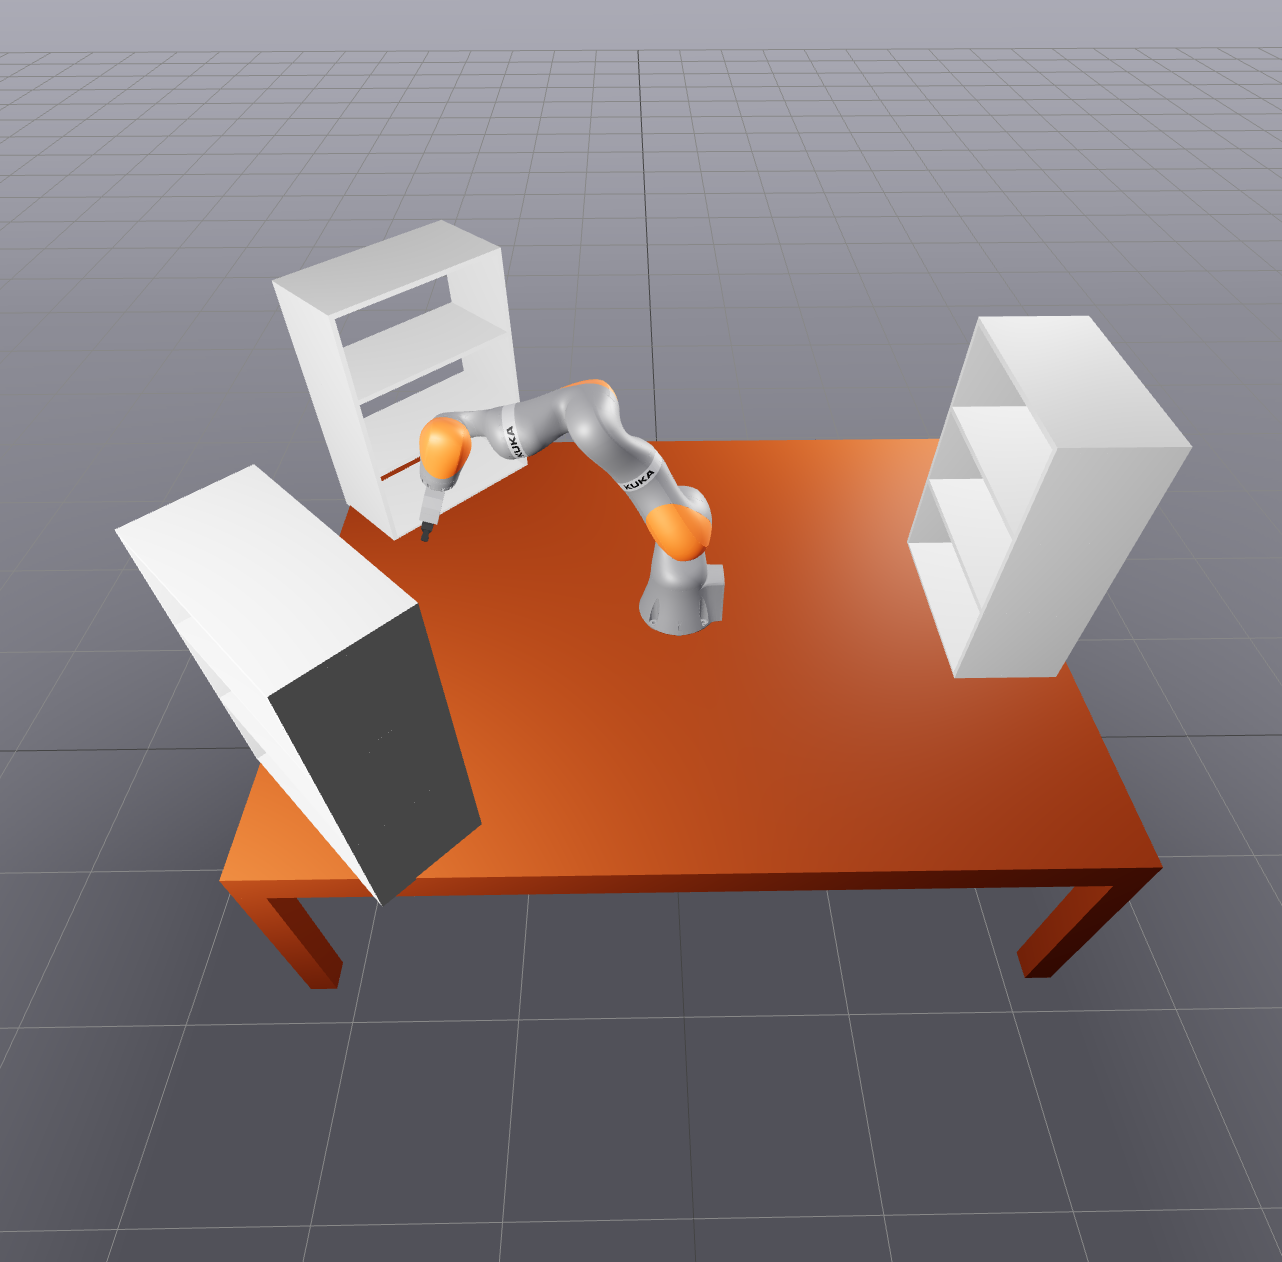
\includegraphics[
            height=3.5cm,
            keepaspectratio
        ]{meshcat3.png}
        \caption{Манипулятор и три полки вокруг него}
    \end{subfigure}

    \caption{Экспериментальные сцены, использованные для построения IRIS-регионов}
    \label{fig:scenes}
\end{figure}

Для каждой сцены выполнялись независимые запуски алгоритма IRIS с числом
начальных точек 10, 20, 30 и 50 (Рис. 2.2). В ходе экспериментов измерялись время
построения выпуклых регионов, количество изолированных регионов, а также
качество покрытия пространства конфигураций. Оценка покрытия выполнялась
методом Монте-Карло на основе 500 случайных конфигураций.
Покрытие определялось как доля конфигураций, принадлежащих хотя бы одному
выпуклому региону.

\begin{figure}[h!]
    \centering
    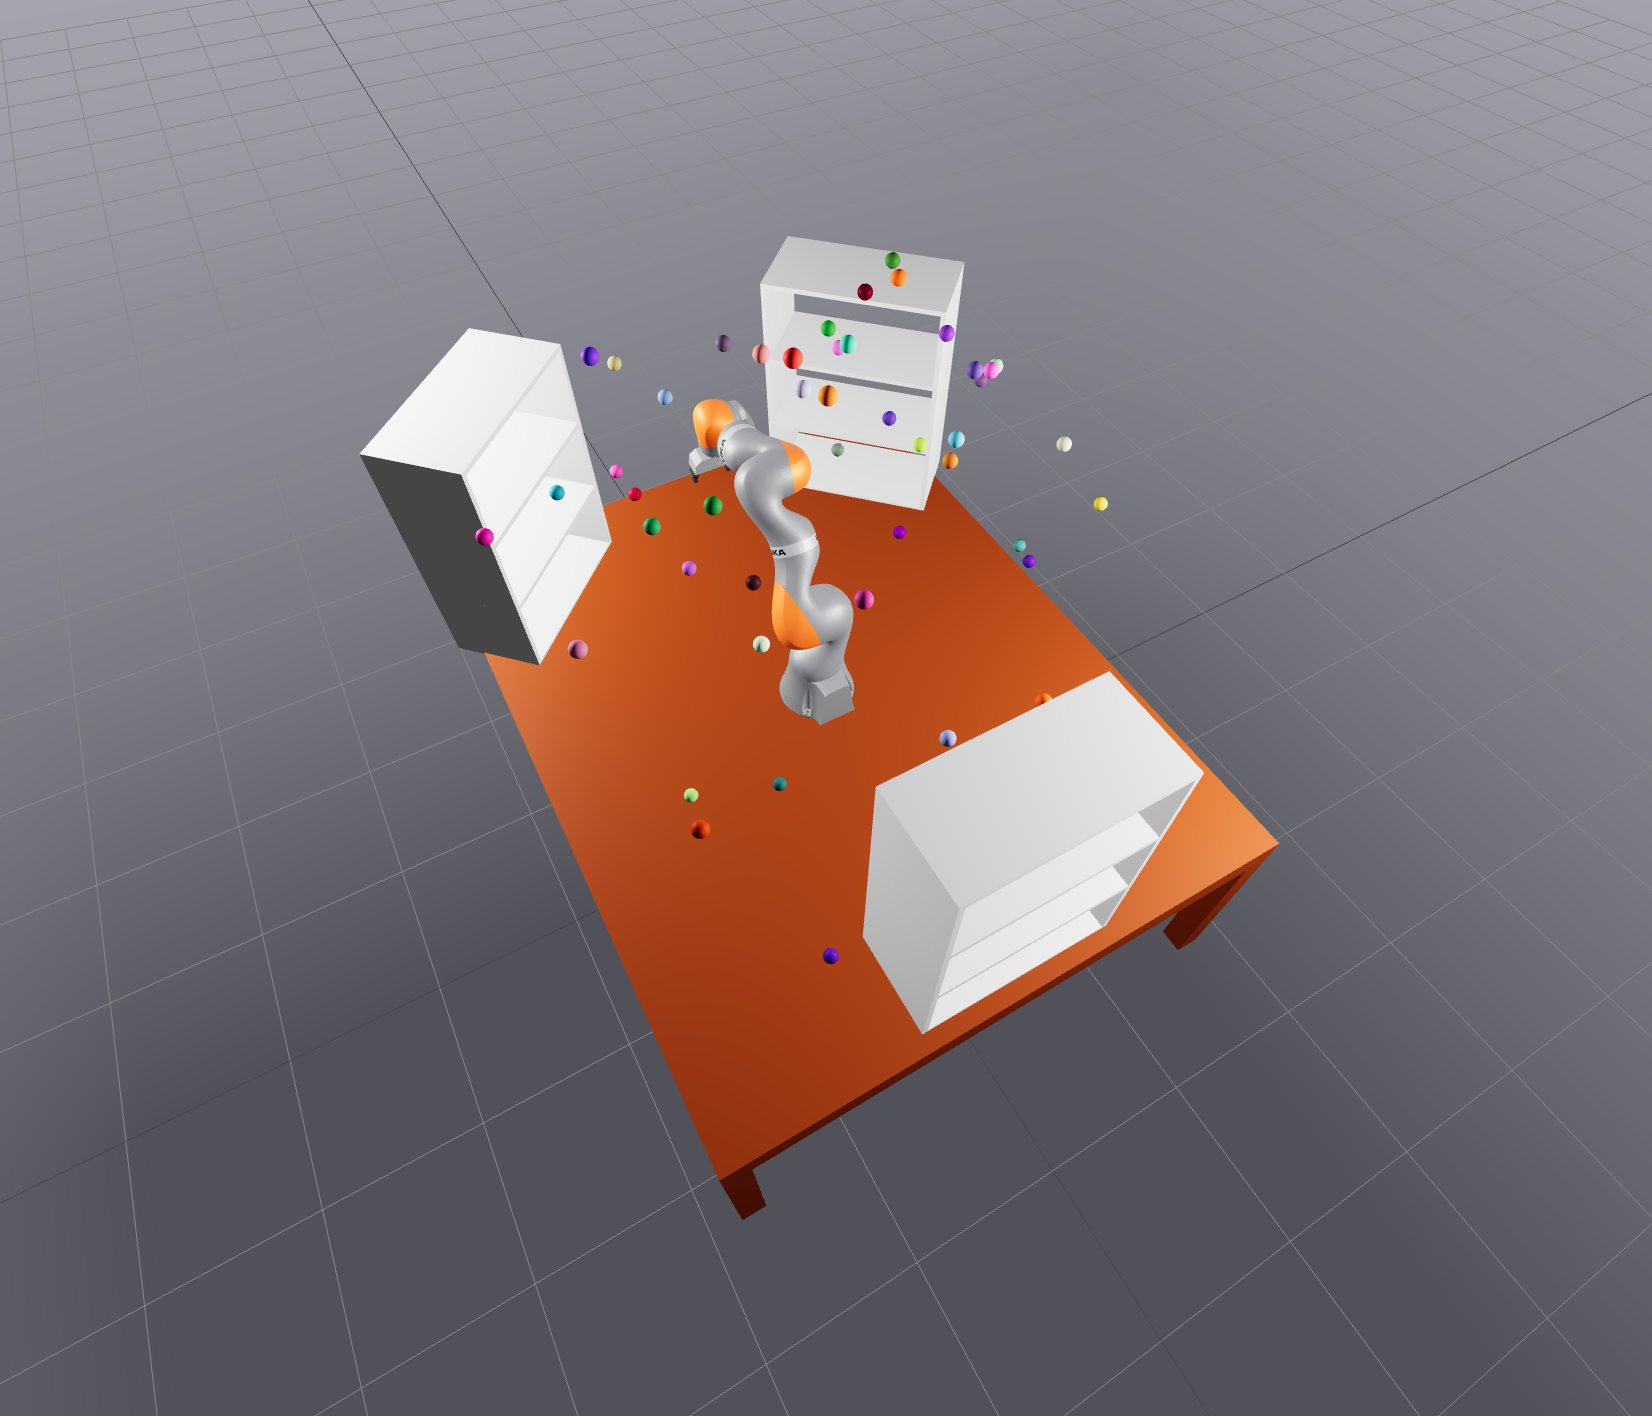
\includegraphics[
        height=6.1cm,
        keepaspectratio
    ]{meshcat_points.png}
    \caption{Случайно сгенерированные начальные точки для алгоритма IRIS}
    \label{fig:iris-seeds}
\end{figure}


\begin{table}[H]
\centering
\caption{Анализ покрытия IRIS-регионами для различных сцен}
\begin{tabular}{lccccc}
\toprule
Scene & Seeds & Isolation (\%) & Coverage (\%) & IRIS Time (s) \\
\midrule
Single Shelf & 10 & 0.0 & 67.0 & 63 \\
Single Shelf & 20 & 0.0 & 67.8 & 156 \\
Single Shelf & 30 & 0.0 & 76.2 & 180 \\
Single Shelf & 50 & 0.0 & 83.0 & 319 \\
\midrule
Two Shelves & 10 & 0.0 & 66.3 & 97 \\
Two Shelves & 20 & 0.0 & 72.2 & 218 \\
Two Shelves & 30 & 0.0 & 75.2 & 256 \\
Two Shelves & 50 & 0.0 & 82.2 & 430 \\
\midrule
Three Shelves & 10 & 0.0 & 40.2 & 348 \\
Three Shelves & 20 & 0.0 & 47.2 & 413 \\
Three Shelves & 30 & 0.5 & 51.5 & 691 \\
Three Shelves & 50 & 0.5 & 60.2 & 1299 \\
\bottomrule
\end{tabular}
\end{table}

Результаты показывают, что увеличение числа начальных точек приводит к росту
покрытия пространства конфигураций, однако при этом существенно возрастает
время построения выпуклых регионов, особенно для сцен со сложной геометрией.
Кроме того, равномерная случайная генерация начальных точек приводит к
недостаточному покрытию узких и геометрически сложных областей сцены,
в частности зон вблизи полок.

\subsection{Эксперименты по планированию траекторий с использованием GCS}

Во второй серии экспериментов исследовалось влияние качества разбиения
пространства конфигураций на результаты планирования траекторий. Для
улучшения покрытия областей сложной геометрии был введён параметр
\texttt{shelf\_ratio}, определяющий долю начальных точек для IRIS,
генерируемых вблизи полок. Во всех экспериментах использовалось значение
\texttt{shelf\_ratio = 0.3}.

Качество планирования оценивалось по двум метрикам: длина траектории и
время решения. Были рассмотрены два сценария: планирование между максимально
удалёнными точками в пространстве конфигураций и планирование между
позициями на полках.

\subsubsection{Планирование между удалёнными точками}

\begin{table}[H]
\centering
\caption{Результаты планирования между удалёнными точками}
\begin{tabular}{lcccc}
\toprule
Scene & Seeds & Success & Path Length & Solve Time (s) \\
\midrule
Single Shelf & 10 & 3/3 & 10.31 $\pm$ 0.20 & 0.007 \\
Single Shelf & 20 & 3/3 & 11.29 $\pm$ 1.00 & 0.012 \\
Single Shelf & 30 & 3/3 & 10.73 $\pm$ 0.62 & 0.008 \\
Single Shelf & 50 & 3/3 & 11.03 $\pm$ 0.46 & 0.007 \\
\midrule
Two Shelves & 10 & 3/3 & 12.93 $\pm$ 1.25 & 0.029 \\
Two Shelves & 20 & 3/3 & 11.81 $\pm$ 1.44 & 0.010 \\
Two Shelves & 30 & 3/3 & 11.00 $\pm$ 0.65 & 0.014 \\
Two Shelves & 50 & 3/3 & 11.06 $\pm$ 1.22 & 0.008 \\
\midrule
Three Shelves & 10 & 3/3 & 9.77 $\pm$ 0.51 & 0.019 \\
Three Shelves & 20 & 3/3 & 10.52 $\pm$ 1.59 & 0.021 \\
Three Shelves & 30 & 3/3 & 10.30 $\pm$ 0.42 & 0.013 \\
Three Shelves & 50 & 3/3 & 10.99 $\pm$ 0.76 & 0.027 \\
\bottomrule
\end{tabular}
\end{table}

Во всех сценах была достигнута 100\% успешность планирования. Время решения
остается малым, что подтверждает эффективность двухэтапного подхода с
использованием предварительного поиска пути в графе регионов.

\subsubsection{Планирование между позициями на полках}

\begin{table}[H]
\centering
\caption{Результаты планирования между позициями на полках}
\begin{tabular}{lccccc}
\toprule
Scene & Seeds & Success & Success (\%) & Path Length & Solve Time (s) \\
\midrule
Single Shelf & 10 & 3/3 & 100 & 0.48 & 0.010 \\
Single Shelf & 20 & 1/3 & 33 & 0.07 & 0.002 \\
Single Shelf & 30 & 1/3 & 33 & 0.18 & 0.002 \\
Single Shelf & 50 & 1/3 & 33 & 0.07 & 0.001 \\
\midrule
Two Shelves & 10 & 0/15 & 0 & -- & -- \\
Two Shelves & 20 & 1/15 & 7 & 0.01 & 0.000 \\
Two Shelves & 30 & 10/15 & 67 & 1.02 & 0.006 \\
Two Shelves & 50 & 0/15 & 0 & -- & -- \\
\midrule
Three Shelves & 10 & 3/21 & 14 & 0.11 & 0.002 \\
Three Shelves & 20 & 11/21 & 52 & 0.56 & 0.001 \\
Three Shelves & 30 & 12/21 & 57 & 0.70 & 0.003 \\
Three Shelves & 50 & 15/21 & 71 & 1.07 & 0.010 \\
\bottomrule
\end{tabular}
\end{table}

Эксперименты в сложных геометриях показали, что увеличение плотности
выпуклых регионов критично для успешного планирования. При этом результаты
остаются нестабильными для некоторых сцен, что указывает на необходимость
дальнейших исследований по улучшению стратегии разбиения пространства конфигураций.


\newpage
\printbibliography[heading=bibintoc]

% Альтернатива ручному оформлению (если требуют thebibliography)
\begin{thebibliography}{0}

\bibitem{lavalle1998}\hypertarget{lavalle1998}{}
LaValle S. M.
Rapidly-Exploring Random Trees: A New Tool for Path Planning //
Proceedings of the IEEE International Conference on Robotics and Automation (ICRA). — 1998.

\bibitem{karaman2011}\hypertarget{karaman2011}{}
Karaman S., Frazzoli E.
Sampling-based algorithms for optimal motion planning //
The International Journal of Robotics Research. — 2011. — Vol. 30. — P. 846--894.

\bibitem{kalashnikov2018}\hypertarget{kalashnikov2018}{}
Kalashnikov D., Irpan A., Pastor P., Ibarz J., Herzog A., Jang E., Quillen D., Holly E.,
Kalakrishnan M., Vanhoucke V., Levine S.
QT-Opt: Scalable Deep Reinforcement Learning for Vision-Based Robotic Manipulation
[Электронный ресурс] //
Proceedings of the 2nd Conference on Robot Learning (CoRL 2018). — Zürich, Switzerland, 2018.

\bibitem{zucker2013}\hypertarget{zucker2013}{}
Zucker M., Ratliff N., Dragan A. D., Pivtoraiko M., Klingensmith M., Dellin C. M.,
Bagnell J. A., Srinivasa S. S.
CHOMP: Covariant Hamiltonian Optimization for Motion Planning //
The International Journal of Robotics Research. — 2013. — Vol. 32. — P. 1164--1193.

\bibitem{marcucci2021}\hypertarget{marcucci2021}{}
Marcucci T., Umenberger J., Parrilo P. A., Tedrake R.
Shortest Paths in Graphs of Convex Sets //
SIAM Journal on Optimization. — 2021.

\bibitem{werner2024}\hypertarget{werner2024}{}
Werner P., Cohn T., Jiang R. H., Seyde T., Simchowitz M., Tedrake R., Rus D.
Faster Algorithms for Growing Collision-Free Convex Polytopes in Robot Configuration Space
[Электронный ресурс] //
arXiv preprint arXiv:2410.12649. — 2024.

\bibitem{werner2024clique}\hypertarget{werner2024clique}{}
Werner P., Amice A., Marcucci T., Rus D., Tedrake R.
Approximating Robot Configuration Spaces with Few Convex Sets using Clique Covers of Visibility Graphs //
Proceedings of the IEEE International Conference on Robotics and Automation (ICRA). — Yokohama, Japan, 2024. — P. 10359--10365.

\bibitem{sucan2012}\hypertarget{sucan2012}{}
Sucan I. A., Moll M., Kavraki L. E.
The Open Motion Planning Library //
IEEE Robotics \& Automation Magazine. — 2012. —
Vol. 19, No. 4. — P. 72--82.

\bibitem{kuffner2000}\hypertarget{kuffner2000}{}
Kuffner J. J., LaValle S. M.
RRT-Connect: An efficient approach to single-query path planning //
Proceedings of the IEEE International Conference on Robotics and
Automation (ICRA). — 2000. — Vol. 2. — P. 995--1001.

\bibitem{solovey2020}\hypertarget{solovey2020}{}
Solovey K., Janson L., Schmerling E., Frazzoli E., Pavone M.
Revisiting the Asymptotic Optimality of RRT //
Proc. IEEE Int. Conf. on Robotics and Automation (ICRA). — 2020. —
С. 2189--2195.

\bibitem{kavraki1996}\hypertarget{kavraki1996}{}
Kavraki L. E., Svestka P., Latombe J.-C., Overmars M. H.
Probabilistic roadmaps for path planning in high-dimensional
configuration spaces //
IEEE Transactions on Robotics and Automation. — 1996. —
T. 12, № 4. — С. 566--580.

\bibitem{kleinbort2019}\hypertarget{kleinbort2019}{}
Kleinbort M., Solovey K., Littlefield Z., Bekris K. E., Halperin D.
Probabilistic Completeness of RRT for Geometric and Kinodynamic
Planning With Forward Propagation //
IEEE Robotics and Automation Letters. — 2019. —
Vol. 4, No. 2.

\bibitem{ratliff2009}\hypertarget{ratliff2009}{}
Ratliff N., Zucker M., Bagnell J. A., Srinivasa S.
CHOMP: Gradient optimization techniques for efficient motion planning //
Proceedings of the IEEE International Conference on Robotics and
Automation (ICRA). — 2009. — P. 489--494.

\bibitem{kalakrishnan2011}\hypertarget{kalakrishnan2011}{}
Kalakrishnan M., Chitta S., Theodorou E., Pastor P., Schaal S.
STOMP: Stochastic trajectory optimization for motion planning //
Proceedings of the IEEE International Conference on Robotics and
Automation (ICRA). — 2011. — P. 4569--4574.

\bibitem{schulman2013}\hypertarget{schulman2013}{}
Schulman J., Ho J., Lee A., Bradlow H., Awwal I., Abbeel P.
Finding locally optimal, collision-free trajectories with sequential
convex optimization //
Proceedings of Robotics: Science and Systems (RSS). — 2013.

\bibitem{toussaint2015}\hypertarget{toussaint2015}{}
Toussaint M.
Robot trajectory optimization using approximate inference //
Proceedings of the International Conference on Machine Learning (ICML). — 2015.

\bibitem{betts2010}\hypertarget{betts2010}{}
Betts J. T.
Practical Methods for Optimal Control and Estimation Using Nonlinear
Programming //
SIAM. — 2010.

\bibitem{dragan2011}\hypertarget{dragan2011}{}
Dragan A. D., Ratliff N. D., Srinivasa S. S.
Manipulation planning with goal sets using constrained trajectory
optimization //
Proc. IEEE Int. Conf. on Robotics and Automation (ICRA). — 2011. —
С. 4582--4588.

\bibitem{elbanhawi2014}\hypertarget{elbanhawi2014}{}
Elbanhawi M., Simic M.
Sampling-Based Robot Motion Planning: A Review //
IEEE Access. — 2014. — Vol. 2. — P. 56--77.

\bibitem{ichter2018}\hypertarget{ichter2018}{}
Ichter B., Harrison J., Pavone M.
Learning Sampling Distributions for Robot Motion Planning //
Proceedings of the IEEE International Conference on Robotics and
Automation (ICRA). — 2018. — P. 7087--7094.

\bibitem{faust2018}\hypertarget{faust2018}{}
Faust A., Oslund K., Francis A., Paxton C., Lu Y., Chen C.,
Liu J., Kew J., Fiser M., Meier F.
PRM-RL: Long-Range Robotic Navigation Tasks by Combining Reinforcement
Learning and Sampling-Based Planning //
Proceedings of the IEEE International Conference on Robotics and
Automation (ICRA). — 2018. — P. 5113--5120.

\bibitem{qureshi2019}\hypertarget{qureshi2019}{}
Qureshi A. H., Yip M. C.
Motion Planning Networks //
Proceedings of the IEEE International Conference on Robotics and
Automation (ICRA). — 2019. — P. 211--217.

\bibitem{wang2020}\hypertarget{wang2020}{}
Wang J., Zhang X., Yu H., Xu K.
Neural RRT: Learning-Based Optimal Path Planning //
IEEE Robotics and Automation Letters. — 2020. —
Vol. 5, No. 2. — P. 2260--2267.

\bibitem{deits2014}\hypertarget{deits2014}{}
Deits R., Tedrake R.
Computing Large Convex Regions of Obstacle-Free Space Through
Semidefinite Programming //
Proceedings of the Workshop on the Algorithmic Foundations of
Robotics (WAFR). — 2014.

\bibitem{petersen2023}\hypertarget{petersen2023}{}
Petersen M., Tedrake R.
Growing Convex Collision-Free Regions in Configuration Space using
Nonlinear Programming //
arXiv:2303.14737. — 2023.





\end{thebibliography}
\addcontentsline{toc}{section}{Список литературы}

	
%\newpage 
%\printbibliography[heading=bibintoc] 

% \begin{thebibliography}{0}
% 	\bibitem{chirkova18}\hypertarget{chirkova18}{}
% 	\href{https://arxiv.org/abs/1810.10927}
% 	{Nadezhda Chirkova, Ekaterina Lobacheva, Dmitry Vetrov. Bayesian Compression for Natural Language Processing. In EMNLP 2018.}
% \end{thebibliography}
	

\end{document}
